\section{Introduction}
\label{sec:introduction}

Every electronic device requires the use of a timing system (usually referred as clock) that sets the reference for the operation of the device.
This timing system is implemented through the use of various electronic components such as clock source, phase comparator, frequency dividers\dots

The aim of this project is to investigate deeply the \acrfull{csac} source technology.

\acrshort{csac} is a type of atomic clock that is designed to be small and low-power, making it suitable for use in portable and battery-powered applications.
% It is based on the principle of coherent population trapping, which is a quantum interference effect that occurs in a three-level atomic system.
Its capability to provide a stable and accurate time reference makes it the optimal choice for a wide range of applications, including satellite navigation, telecommunications, and military systems.

\begin{figure}[H]
    \centering
    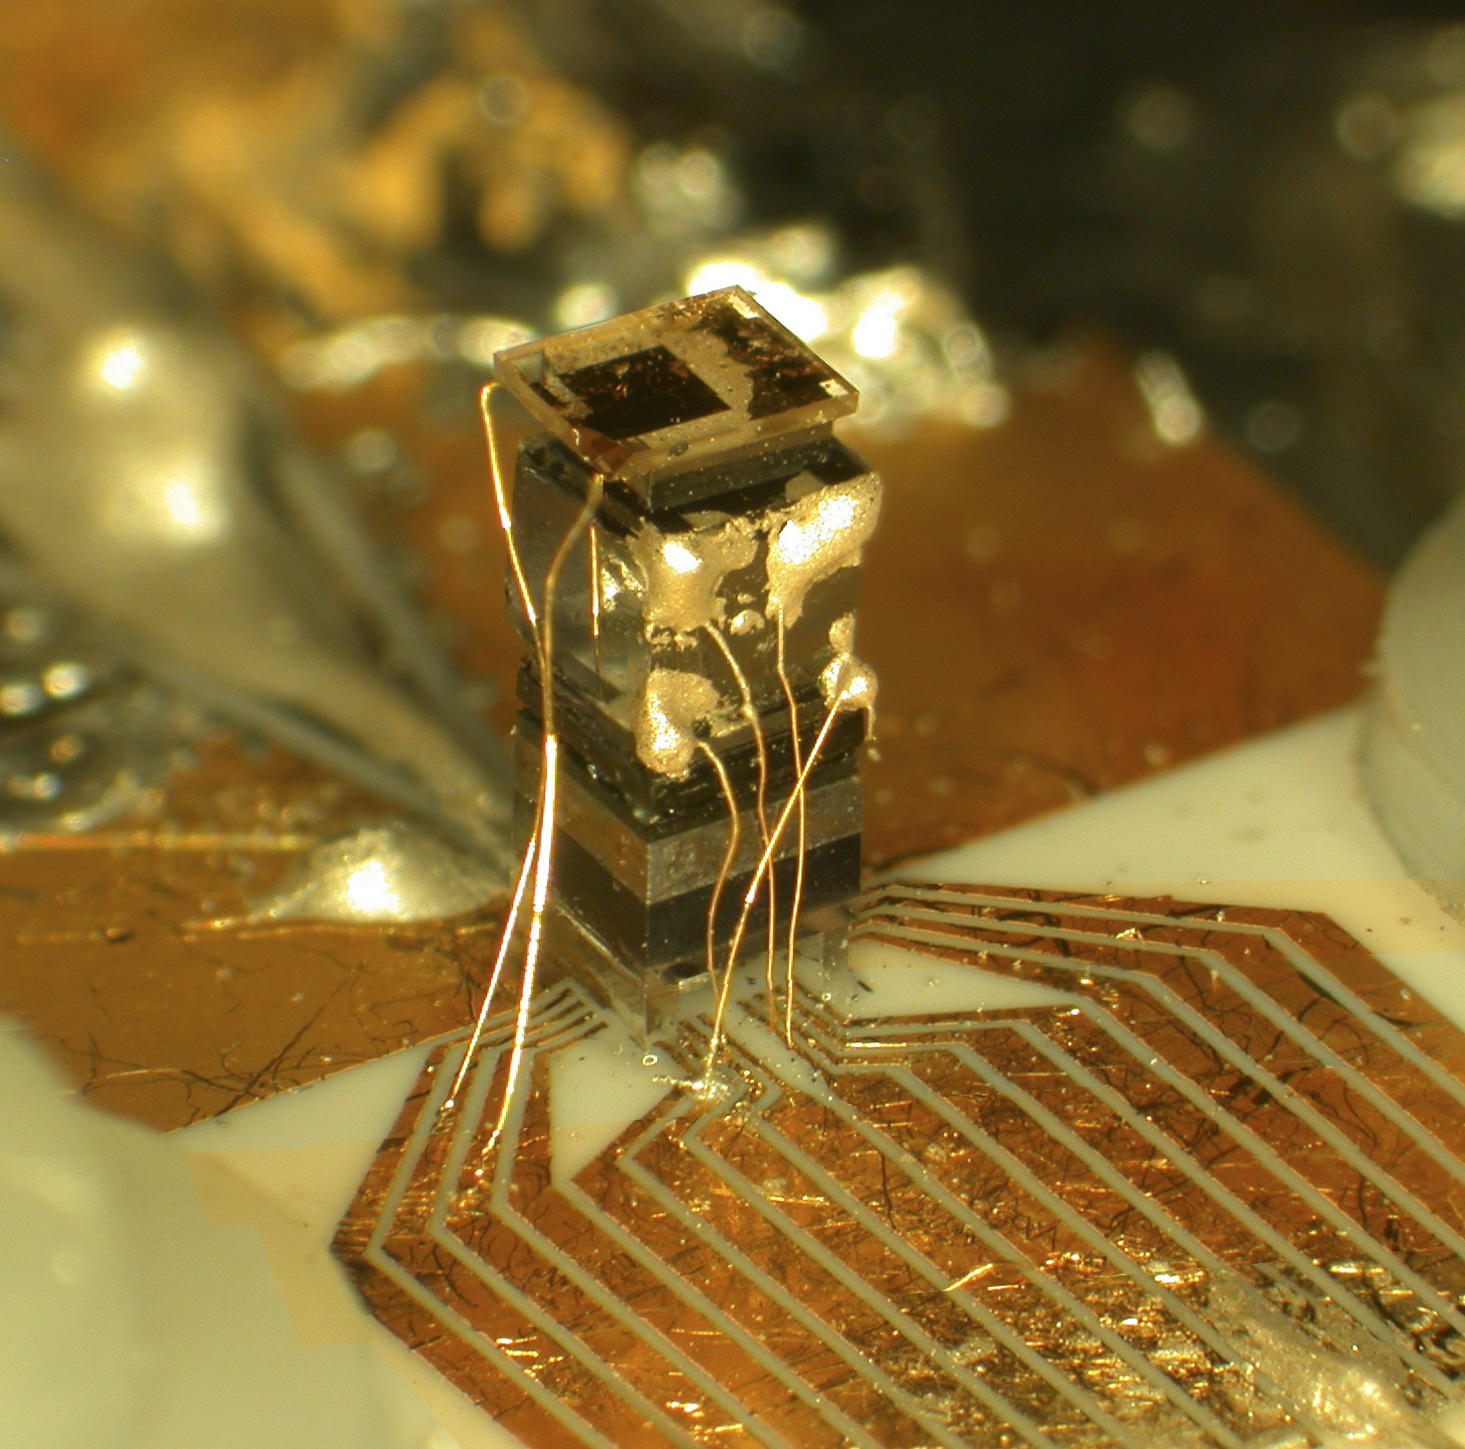
\includegraphics[width=.5\textwidth]{img/first_atomic_clock.jpg}
    \caption{\href{https://www.nist.gov/news-events/news/2004/08/nist-unveils-chip-scale-atomic-clock}{NIST chip-scale atomic clock.}}
\end{figure}

\begin{figure}[H]
    \centering
    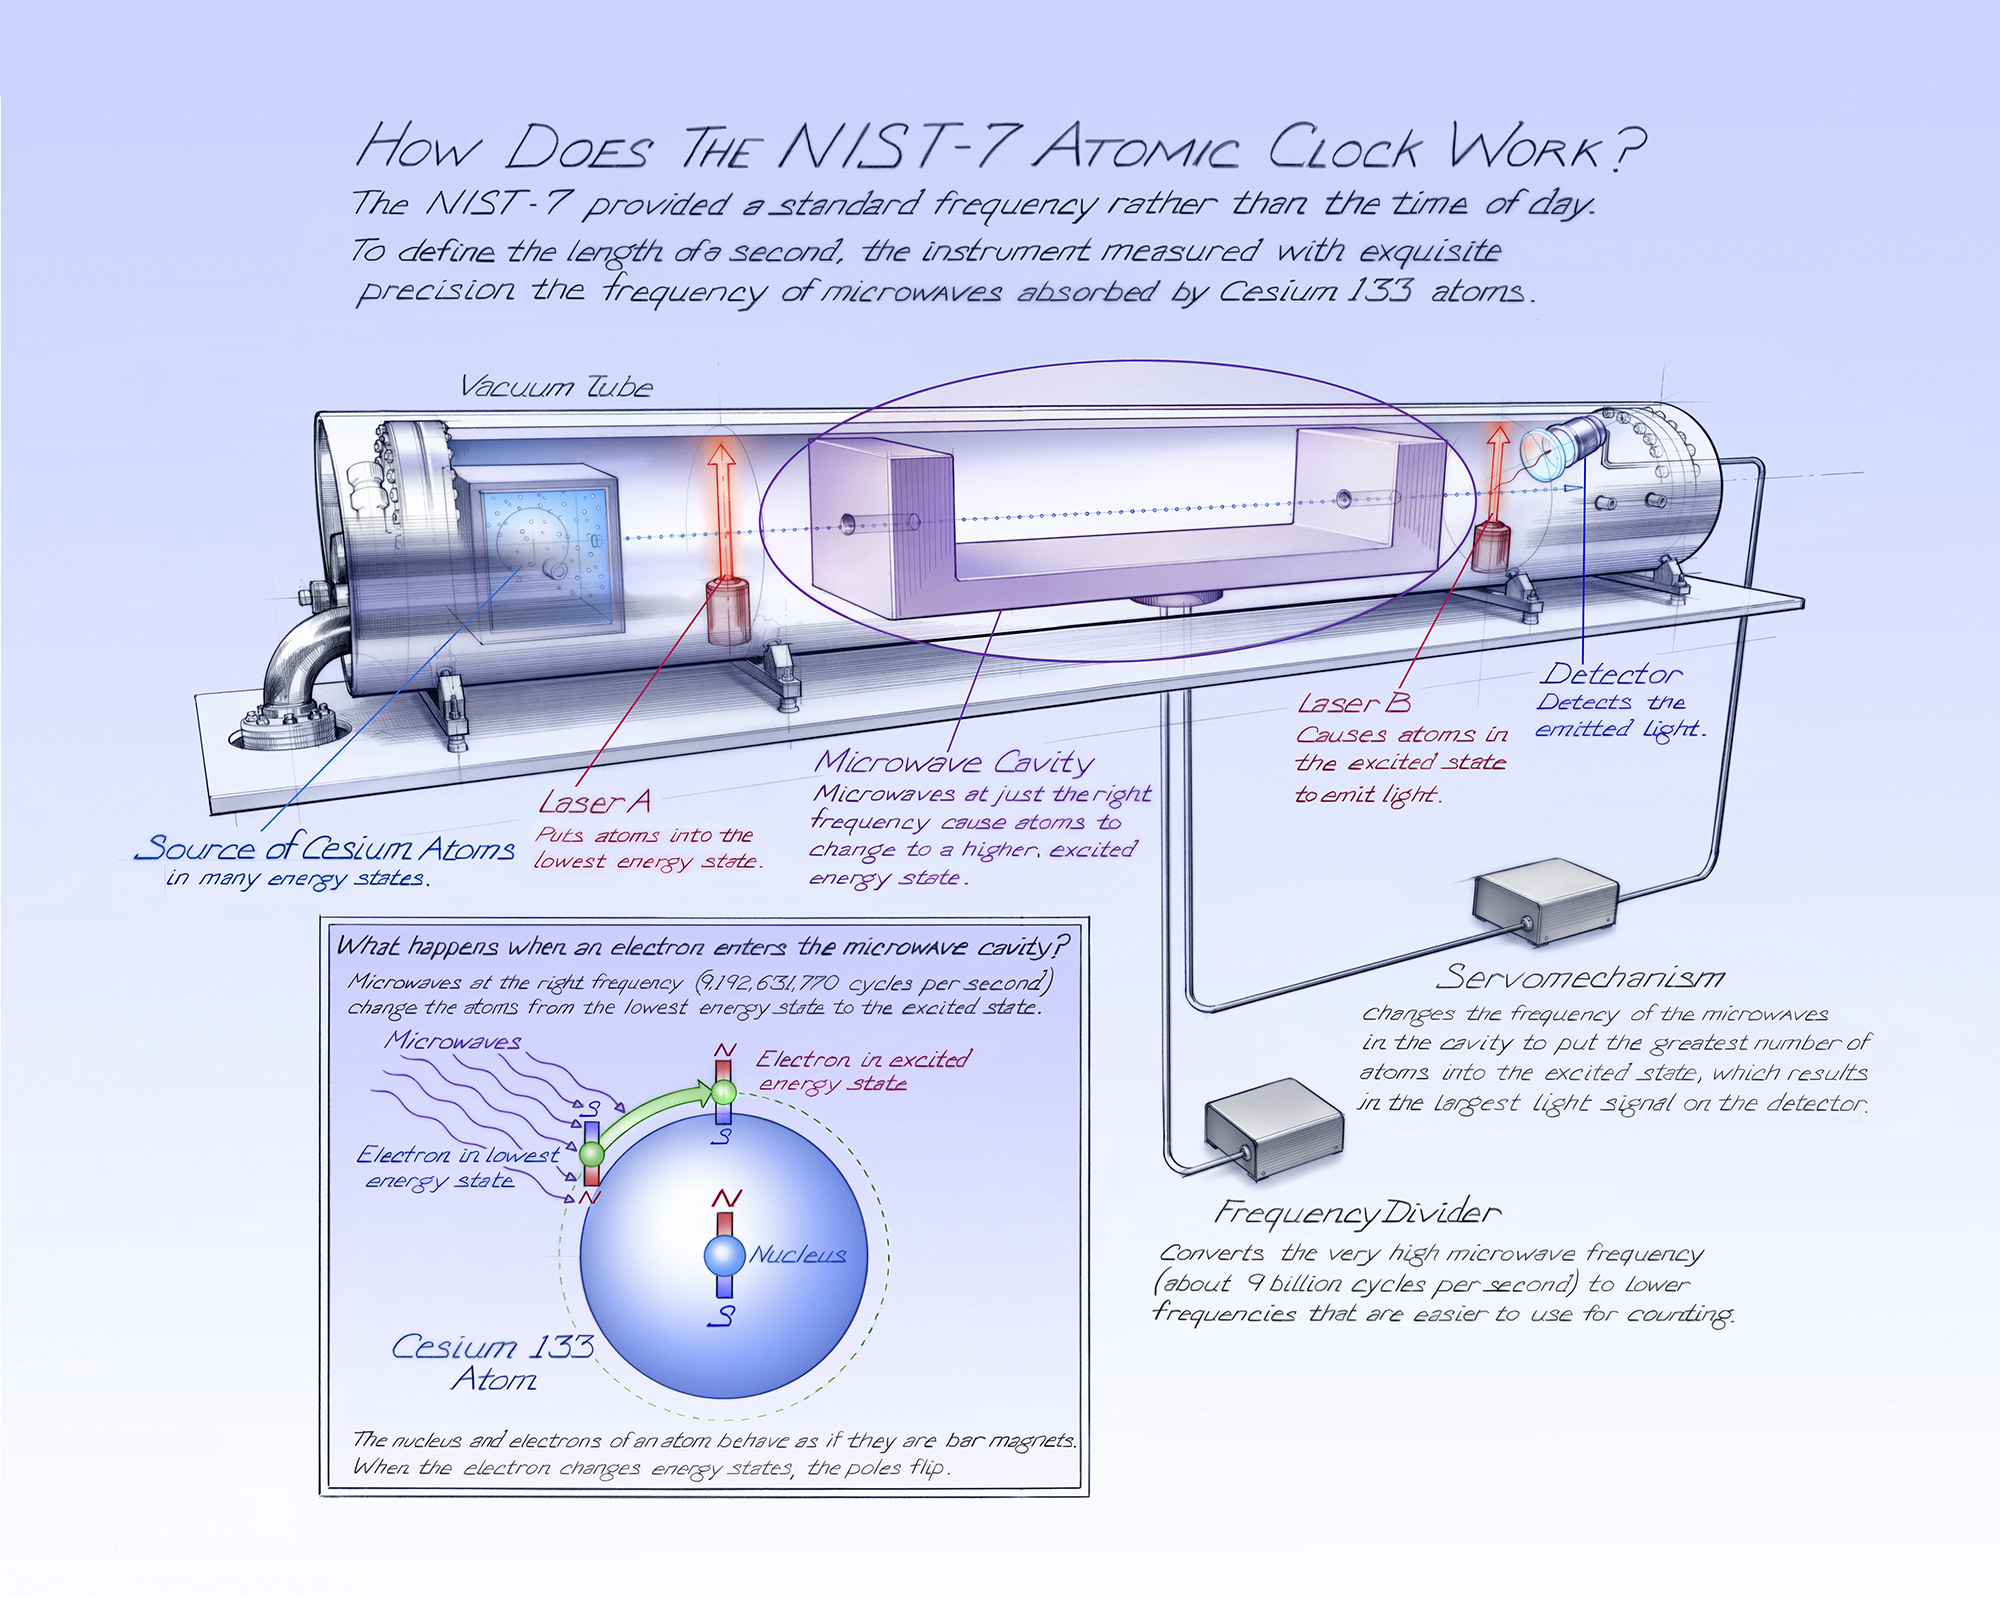
\includegraphics[width=.6\textwidth]{img/cesium_atomic_clock_scheme.jpg}
    \caption{\href{https://timeandnavigation.si.edu/multimedia-asset/how-does-the-nist-7-atomic-clock-work}{NIST-7 atomic clock scheme, credit Bruce Morser}}
\end{figure}
